\documentclass[11pt,a4paper,titlepage,oneside]{report}

\usepackage[english]{babel}
\usepackage[utf8]{inputenc} % input encoding is UTF-8

\usepackage{graphicx}
\usepackage{tabularx}

\usepackage{color}
\usepackage[unicode,pdftex]{hyperref}

\begin{document}

% Title page %%%%%%%%%%%%%%%%%%%%%%%%%%%%%%%%%%%%%%%%%%%%%%%%%%%%%%%%
\begin{titlepage}

\begin{center}

\includegraphics[width=0.5\textwidth]{img/logo_NTNU.png}\\
\vfill
{\LARGE \textbf{TDT4290 - Customer Driven Project}}
\vfill
{\Huge \textbf{Ocean forecast}}

\vspace{12pt}
{\LARGE \textbf{SINTEF}}

\vspace{30pt}
{\LARGE \textbf{Pre study}}
\vfill
{\LARGE \textbf{Autumn 2014}}
\end{center}
\vfill
\begin{tabular*}{\textwidth}{@{\extracolsep{\fill}} l l}
\textbf{Group 6} & \textbf{Advisor} \\
Arve Nygård & Gleb Sizov \\
Anders Smedegaard Pedersen & \\
Emil Jakobus Schroeder & \\
Hans Kristian Henriksen & \\
Marco Radavelli & \\
Ondřej Hujňák & \\
Ruben Håskjold Fagerli & \\
\end{tabular*}

\end{titlepage}

% Empty page %%%%%%%%%%%%%%%%%%%%%%%%%%%%%%%%%%%%%%%%%%%%%%%%%%%%%%%%
\newpage
\thispagestyle{empty}
\mbox{}
\newpage

% Abstract %%%%%%%%%%%%%%%%%%%%%%%%%%%%%%%%%%%%%%%%%%%%%%%%%%%%%%%%%%
\begin{abstract}
Na na na na na na na, Batman!!!
\end{abstract}

% Signatures %%%%%%%%%%%%%%%%%%%%%%%%%%%%%%%%%%%%%%%%%%%%%%%%%%%%%%%%
\thispagestyle{empty}
\begin{center}
{\large \textbf{Trondheim, \today}}\\
\vspace{2.5cm}
\begin{tabularx}{\textwidth}{@{\extracolsep{1cm}} X X }
\dotfill & \dotfill \\
~Arve Nygård & ~Anders Smedegaard Pedersen \\[1cm]
\dotfill & \dotfill \\
~Emil Jakobus Schroeder & ~Hans Kristian Henriksen \\[1cm]
\dotfill & \dotfill \\
~Marco Radavelli & ~Ondřej Hujňák \\[1cm]
\dotfill & \\
~Ruben Håskjold Fagerli & \\[1cm]
\end{tabularx}
\end{center}

% Table of contents %%%%%%%%%%%%%%%%%%%%%%%%%%%%%%%%%%%%%%%%%%%%%%%%%
\tableofcontents
\addtocontents{toc}{\protect\thispagestyle{empty}}

% List of figures %%%%%%%%%%%%%%%%%%%%%%%%%%%%%%%%%%%%%%%%%%%%%%%%%%%
\listoffigures
\addtocontents{lof}{\protect\thispagestyle{empty}}

% List of tables %%%%%%%%%%%%%%%%%%%%%%%%%%%%%%%%%%%%%%%%%%%%%%%%%%%%
\listoftables
\addtocontents{lot}{\protect\thispagestyle{empty}}

\pagenumbering{arabic}
\setcounter{page}{0}

% Main body %%%%%%%%%%%%%%%%%%%%%%%%%%%%%%%%%%%%%%%%%%%%%%%%%%%%%%%%%
%%%%%%%%%%%%%%%%%%%%%%%%%%%%%%%%%%%%%%%%%%%%%%%%%%%%%%%%%%%%%%%%%%%%%

\chapter{Introduction}
\section{TDT 4290 - Customer driven project}
The task is set forth in the subject TDT 4290 - Customer driven project at the Norwegian university of science and technology. The goal of the course is 
\begin{quote}
(...)to give the students a practical experience of carrying out all the phases of a typical customer guided IS/IT-project. \cite{TDT4290:Intro}
\end{quote}
The subject divides the students into random groups, and assigns each group an assignment. The assignments are real problems that businesses needs solved. 

Although the assignment is to follow the entire process of an IT-project, the focus is on the earlier phases of a project. Thus, an important part of the assignment is the work leading up to the implementation phase.

\section{Pre study}
To get an understanding of the customers needs, as well as studying different solutions, a pre study is conducted. From the course compendium:
\begin{quote}
The preliminary studies are vital for the group to obtain a good understanding of the total problem.
Here, you will have to describe the problem at hand. You should describe the current system and the
planned solutions (...).
\end{quote}

The report is produced to formalise the recommendation that is made to the customer. Although the report contains the entire background and recommendation, the customer has been kept up to date with the work, and been presented with our conclusions well before this study was finished. This has been necessary for our work to continue, and was agreed upon with the customer in advance.

\section{Work organisation}
In this first work period, we have worked in two phases. For the first phase, we worked with the goal of familiarising ourselves with the file format, and the technology. In this period the group was divided into two groups, one investigating the front end, and one the back end. For the second phase, the group adopted the scrum methodology, and used one sprint to finish the recommendation. 


\chapter{Assignment and use cases}
This chapter will give a brief description of the assignment given to the group, the problem domain, as well as some example use cases. 
\section{Domain}
The groups assignment is connected to SINTEFs work on oceanographic simulations. By analysing large amounts of observational data, and running this trough complex simulations, the goal is to predict future conditions. 

More specifically, the currents, temperature, salinity and other factors are recorded, simulated and predicted. These predictions are used mainly by stakeholders in the fish farming industry for decision support. Usually this is in conjunction with lice removal, which requires precise positioning of large supply vessels. 

\section{Assignment}
The assignment set forth by SINTEF is to improve the current solution to be able to serve the user with dynamically created views of the data. 
\section{Use cases}

\chapter{Current situation at SINTEF}
In this chapter we will explore the solution SINTEF is currently using, and the challenges and limitations it poses. After looking into this, we will describe the evaluation criteria that will be used to assess the alternative solutions the group has found. 
\section{Current system}
\begin{figure}[h]
\begin{center}
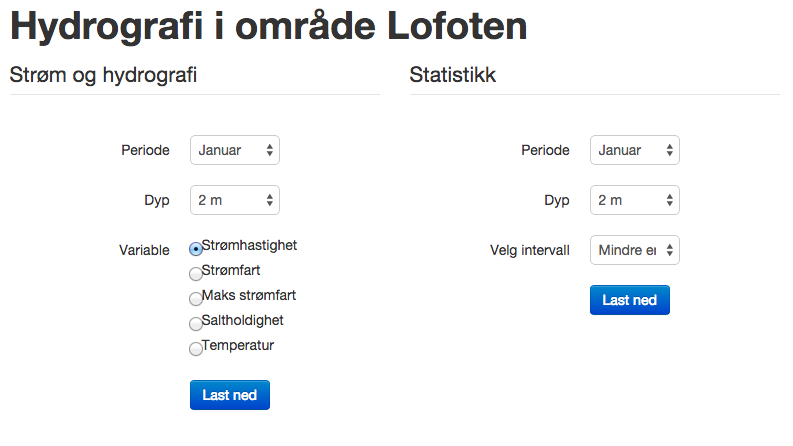
\includegraphics[height=223px,width=396px]{img/region_interface_sinmod.png}
\caption{The main interface for a region in SinMod}
\label{fig:sinmod-region-main-interface}
\end{center}
\end{figure}

The current system deployed at SINTEF serves their clients by providing access to a collection of more than 100 000 pre generated PDF files. These files contain information on currents, salinity, and temperature. The user may choose what information he wants by selecting parameters in the drop down menus, see figure \ref{fig:sinmod-region-main-interface}.

\begin{figure}[h]
\begin{center}
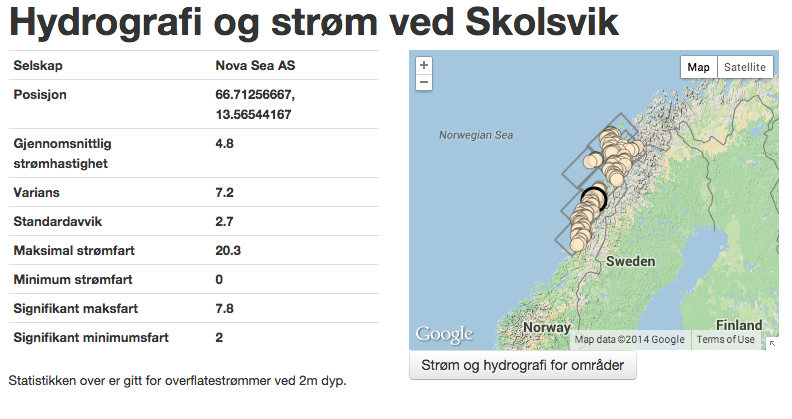
\includegraphics[height=223px,width=396px]{img/site_key_data.png}
\caption{The key data a user is presented with when selecting a specific site}
\label{fig:sinmod-site-key-data}
\end{center}
\end{figure}

If the user chooses a specific site from the map or location drop down, he will be presented with key data for this area. This includes statistical information such as maximum current speed, average current speed and so forth, as well as geographical position, as given in figure \ref{fig:sinmod-site-key-data}.


\begin{figure}[h]
\begin{center}
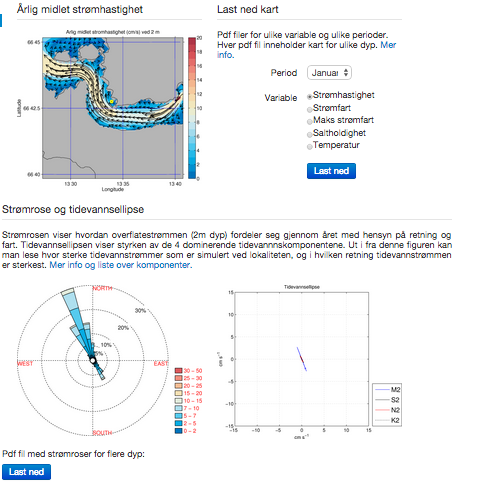
\includegraphics[height=300px,width=300px]{img/site_graphs.png}
\caption{The graphs presented to the user when selecting a specific site}
\label{fig:sinmod-site-graphs}
\end{center}
\end{figure}

The system will also present a set of pre defined graphs, including current roses, tidal ellipsis and vertical profiles. The graphs are given for standard attributes (e.g depth 2 meters), and for some of them, there is an option of downloading a PDF containing graphs for other values of the given attributes. An example is shown in figure \ref{fig:sinmod-site-graphs}


\section{Challenges}
As the PDFs are pre generated, there is a clear limitation to what information the user may request. If a user wants to know, for example, the connection between salinity and current speed at a given location, the user must download two different PDFs and manually compare these. 

The graphs given for a specific location are only given for limited values of the critical attributes. If we look at the current rose, it is presented for a depth of 2 meters. If the user is really interested in the current rose for 10 meters, he has to download the PDF containing all possible current roses. 

The same is true for the maps that can be generated for a specific site. The user may choose period (a single month may be selected), and one of the five variables. This gives the user a PDF with one map for each depth that can be calculated. 

For a user that knows what data is interesting, this is a complicated and data heavy way of delivering information. The PDFs seems to range in size from 125kB to around 3MB, depending on what information is requested. The region maps are the absolute largest in file size, ranging from 1 to 3MB, while the files containing the current roses are quite small, in the 100-200kB range. 

On a computer with broadband connection, the size of the files is not very problematic. For these users, the biggest challenge is the fact that the user can not specify what kind of data they want plotted, and have to look through quite a lot of pages to get the information needed. For a user on a low bandwidth connection and/or on a mobile device, the size of the files is a more pressing problem. On an EDGE connection the theoretical best download time for a 3MB file is 62,5 seconds at 384kbit/s \cite{3gpp.com}.

\section{Evaluation criteria}
SINTEFs main goal with this project is to be able to rid themselves of the PDF store, and generate the information on demand. This will make for a much more flexible system, where it will be possible to add new graphs and functionality quickly. For the customers, it will make it possible to request more customised graphs and plots.

SINTEF has presented the group with several goals they wish the new system to fulfil:

\begin{itemize}
\item The system should generate the graphs and maps directly from the NetCDF files on user request.
\item The user should be able to select several variables for one plot.
\item The system should be usable on low bandwidth connections.
\item The system should be usable on mobile devices.
\item The system should be easy to expand with new functionality.
\end{itemize} 

With these goals in mind, the group started looking into different technologies that could be used to make such a system.

%%%
\chapter{Other production solutions}
The group has used the first part of the project investigating what solutions would best suit SINTEFs needs. In the chapter we present the different solutions we have found, along with an assessment on how each solution is rated in accordance to the evaluation criteria. 

%Existing tech - Italian solution
\section{Adriatic Forecasting System}
\emph{Link: \url{http://oceanlab.cmcc.it/afs/}} \\%make sure to use //
  The solution, by the Operational Oceanography Group Italy and cmcc Ocean-Lab, can display temperature, salinity, currents, sea surface height, wind stress and heat flux. It allows to choose date, region and depth as search filters, and uses PNGs on a Google map. The PNGs are retrieved from cmcc's own server.
  Although it seems nice to look graphically, it can be seen that some tiles are not precisely overlapping. In addition, sometimes is needed to refresh the page because the application doesn't load properly. PNGs layers are displayed without a specific JS library, and the JS code is quite complex compared to other existing solutions using libraries. Therefore this solution is not well re-usable.
\\ \emph{Overall rating: \textbf{Ok}}

\section{Danish Centre of Ocean and Ice}
  \emph{Link: \url{http://http://ocean.dmi.dk/anim/index.uk.php }} \\%make sure to use //
    The solution by the Danish Center of Ocean and Ice can display temperature, salinity and current which are the most important factors of the Sintef simulation. This said it lacks the ability to choose depth and specify a date interval. The data is shown as static PNGs, thus the map is not interactive. There is, on the other hand, a posibility to choose different geographical areas with the highest level of detail around Denmark. This is on the same level as Sintef's excisting solution.
  \\ \emph{Overall rating: \textbf{Bad}}

  \section{Fisheries and Oceans Canada}
  \emph{Link: \url{http://www.tides.gc.ca/eng}} \\%make sure to use //
    The solution of the Canadian government resembels the Danish one. It is possible to choose a geographical area on a static map. By choosing an area you get the oppotunity to choose a smaller, more sepcific area. The bug difference is that all data is presented as text in tables, thus making it less convinient and intuitive to use.
  \\ \emph{Overall rating: \textbf{Bad}}

  \section{Ocean viewer}
  \emph{Link: \url{http://www.oceanviewer.org}} \\%make sure to use /
    Ocean Viewer is a pilot project of the Marine Environmental Observation Prediction and Response Network (MEOPAR) of Canada. It gathers data from different sources and displays it as PNGs overlayed on a map. You can select different geographical areas on a customized Google Map and different data from a menu (temperature, salinity and others). Like the Danish solution the PNGs can be shown in sequence to show changes over time.
  \\ \emph{Overall rating: \textbf{Ok}}

  \section{Sea temperatures and Currents - Bureau of Meteorology}
  \emph{Link: \url{http://www.bom.gov.au/oceanography/forecasts/}} \\%make sure to use //
    The Australian Bureau of Meteorology has a solution that is very similar to the other national agencies. You can choose a geographical area on a static map. Also here the data is visualized with images overlayed on a static map, with the posibility to loop through the images to show changes in the data over time.
  \\ \emph{Overall rating: \textbf{Ok}}
  
  \section{yr.no Map Service}
  \emph{Link: \url{http://yr.no/kart}} \\%make sure to use //
This solution presents the user with a conventional map interface. On the sides and top there are menus for selecting which variable and timestep should be displayed. The user is only allowed to select a timestep about 8 days from the current time. Interesting variables include sea temperature, salinity and sea currents, each has it’s own . There is no way to select depth, and all data seems to be for the surface values. The chosen variable is added as an overlay of png tiles using OpenLayers. The tiles are fetched using WMS from a norwegian meteorological service server. On the map there are several measurement stations displayed, that give information when clicked. In addition, clicking anywhere on the map displays several plots predicting the next two days of weather for that spot.
  \\ \emph{Overall rating: \textbf{Ok}}

\chapter{Back-end}

  \section{GeoServer}
  Does not support NetCDF natively. There exist a community plugin that enables you to read from NetCDF files, but the support seems very shifty. Does not seem to have support for more than one file and metadata looks like a pain to extract. Further investigation was aborted.

  \section{THREDDS}
  \begin{quote}
  The THREDDS\footnote{\textbf{Th}ematic \textbf{R}ealtime \textbf{E}nvironmental \textbf{D}istributed \textbf{D}ata \textbf{S}ervices} Data Server (TDS) is a web server that provides metadata and data access for scientific datasets, using OPeNDAP, OGC WMS and WCS, HTTP, and other remote data access protocols. \cite{TDS:Web}
  \end{quote}

  Except supporting multiple data access protocols, TDS is able to virtually aggregate multiple netCDF files to one dataset that can be used for queries such as selecting a region and sending it's data in specified format. Dataset configurations are done via NcML\footnote{\textbf{N}et\textbf{C}DF \textbf{M}arkup \textbf{L}anguage}, which is a dialect of XML.

  Although TDS seems to support everything that is needed for this project, it's installation and especially configuration for agreggation and special needs is quite complicated. Moreover there are doubts about speed and dealing with serving a range containing large quantitied of points. Advantage is, that SINTEF currently have a TDS running and configured, so we won't need to configure it from scratch and SINTEF employees probably have experience and knowledge about setting it up which we lack.

  \section{Custom solution}
  An alternative is to write a custom back-end from scratch.
  Advantages of this are:
  \begin{itemize}
  \item Easy deployment - written as a single service that you just launch. One file.
  \item Load balancing - Easily scale outwards: Just put the servers behind a load balancer.
  \item Speed - No overhead for unused features
  \item Code clarity - No overhead for unused features
  \item Extensability - see above \ldots
  \end{itemize}
  A skeleton for the whole server is in place. Below is a list of features that are within reach in the project period. 
  The following features are not finished yet, but have a placeholder as of now:
  \begin{itemize}
  \item Indexing / file selection ( Use Lucene for this)
  \item Projection (Mappign between Lat/Long and file indices)
  \item Filtering (Reducing the result set / density before reading the file)
  \item Output
  \item Rendering to image (map) (Almost finished)
  \item Rendering to GeoJSON (Almost finished) \ldots
  \end{itemize}

  Performance seems to be very good at the current level of implementation. The only major potential bottleneck I see is reading files from a hard-drive. (All testing has been done on SSDs). This bottleneck is independent of backend solution, however.
  
  \section{MapTiler}
  \emph{Link: \url{http://www.maptiler.org/}} \\%make sure to use //
    MapTiler is an application for online map puplishing. It makes it possible to create tiles that can be overlayed over other maps like Google Maps, Open Street Map and others. It's written in C/C++ and claims to be a lot faster than other existing solutions. A draw back seems to be that it's made for overlaying a pre generated directory of images rather than dynamic data like the ocean forecast data.
  \\ \emph{Overall rating: \textbf{Bad/Ok/Good/Very Good}}
  
    \section{ncWMS}
  \emph{Link: \url{http://www.resc.rdg.ac.uk/trac/ncWMS/}} \\%make sure to use //
  	\paragraph{Introduction}
    ncWMS is an open source, free to use, java server application. It was created to support interactive browsing of gridded four-dimensional netCDF data over the web. Clients will send request containing the wanted coordinates (latitudes, longitudes, depth and time), what variable is to be displayed, projection, format and size the response should be. ncWMS, which has been configured to read from datasets (for example sets of netCDF files or a THREDDS server), responds to a request with an image of the desired type. ncWMS adheres to the WMS specification (WMS 1.3.0 and 1.1.1 are supported).
    \paragraph{Configuration}
    ncWMS is mainly configured through a web interface, where you can add datasets and change server settings. A dataset can be: a single netCDF file, an OPeNDAP endpoint (a service provided by THREDDS), a NcML file or a glob aggregation (using wildcard characters like ). It is possible to configure which variables of a dataset to expose and how. Each dataset can also be set to automatically refresh at certain intervals. The server can be set to cache data, to reduce cpu load at the expense of memory and disk space.
    \paragraph{Aggregation}
    The glob aggregation or NcML work well with files that cover the same area, but contain different timesteps. To handle different areas and different resolutions it may be possible to use THREDDS/OPenDAP or NcML.
    \paragraph{Perfomance}
    Testing both local and publicly available ncWMS servers the performance seems good. When using the godiva2 browser based client or sending individual requests the server mostly responds quickly, with some idiopathic exceptions. Transmitting the map data to the client as png images should be a bandwidth-efficient way to do it, as well as moving the computation load away from the client. When starting the server application or adding a dataset, the server needs some time to load some information from the datasets. This only takes a few seconds, even for a few hundred GB of local netCDF files.
    \paragraph{Summary}
    ncWMS does a lot of what we need the back-end of our solution to do. It handles the extraction, downsampling and projection of the data, creating an image ready to be used in a map widget or on it’s own. It can only handle requests for a few kinds of plots. It is open source, and is free to use under a modified BSD license. To serve all the plots and data required it would need modification.
  \\ \emph{Overall rating: \textbf{Good}}


  
%%%
\chapter{Frontend solutions}
  A central part of the product requirement is an to display simulated data in a dynamic manner. There exists solutions to do just that, and javascript libraries than makes it relativly easy to creat at front end solution of our own. In this section we will discuss and compare the most relevant of these in the context of our assignment and the product requirements. 
  \section{Custom made solution}
    A custom made solution has the general advantage that we can built it to specification and thus make sure it meets the requirements without having to deal with other peoples code base. Trying to customize an exisitng solution might be as much work as builting something from the bottom. In the following paragraphs we will review and rate technologies we found relevant for building a custom front end.
    \subsection{LeafletJS}
    \begin{tabular}{|p{4cm}|p{8cm}|}
      \hline
      Home page: & \url{http://www.leafletjs.com} \\
      \hline
      Service functionality: & Creating mobile-friendly interactive maps. \\
      \hline
    \end{tabular}
    
    \paragraph{Introduction} \indent
    LeafletJS ("Leaflet" for the rest of the section) is an open source javascript library for creating mobile-friendly interactive maps. it's licenced under the \href{'https://github.com/Leaflet/Leaflet/blob/master/LICENSE'}{2-clause BSD License}, which makes it free to use in comercial applications as long as a credit is added somewhere in the user interface.
    Even though Leaflet is free to use it is dependant on a third party to provide the map tiles. These may not be free to use.

    \paragraph{Features}
    Leaflet has the features you'd expect from a modern interactive map. This includes paning with inertia, zooming and the ability to add markers. It also supports double-tap and pinch to zoom for IOS and Androidon mobile phones. Furthermore all the five biggest web browsers are supported, including graceful fallback for old versions.
    The most powerful feature of Leaflet is the ability to add layers. 
    \newline The different supported layers are:

    \begin{itemize}
      \item Tile layers
      \item Marker layers
      \item Pop-ups
      \item Vector layers
      \item GeoJSON layers
      \item image overlays
      \item WMS layers
      \item Layer groups
    \end{itemize}

    For our purposes the ability to get map tiles from different sources may be very interesting. This gives us the ability to for example show both nautical maps and regular land maps at the convenience of the user. At zoom levels covering large geographical areas it will probably be most ideal to show the relevant simulated data as overlayed PNGs. This is easily achieved with image overlays in Leaflet. If we want to show very detailed data when zoomed further in, we might be able to use vector layers to visualize the data. It is also possible to use a GeoJSON layer to convert data formatted as GeoJSON to vectors.
    It is also possible to use Web Map Service (WMS) to overlay, for example, metrological data on a map. Eventhough this is a format that is used by large organizations like the National Oceanic and Atsmopheric Administration (\url{noaa.gov}) we have been advised against using this format due to it's negative effect on the speed and responsiveness experieced by the end-user. \footnote{Cite the guy Marco talked with at Yahoo}
    Furthermore Leaflet can be extended with plugins. These can relatively easily be written in Javascript or an excisting plugin can be downloaded and used. A relevant plugin to our needs could for exmaple be heatmap.js (\url{http://www.patrick-wied.at/static/heatmapjs/}).

    \paragraph{Summary}
    Leaflet is very suitable for our needs in respect to creating an interactive map overlayed with visualizations of relevant data created by the Sintef ocean forecast simulations. It's lightweight(33 kilobytes), made to be compatible with mobile phones and very flexible in possibilities to display data on maps. It's also well documented.

  \subsection{OpenLayers}
   \begin{tabular}{|p{4cm}|p{8cm}|}
     \hline
     Home page: & \url{http://openlayers.org/} \\
     \hline
     Service functionality: & A high-performance, feature-packed library for all your mapping needs. \\
     \hline
   \end{tabular}
   \paragraph{Introduction} \indent
   OpenLayers is an open source (provided under the \href{'https://github.com/Leaflet/Leaflet/blob/master/LICENSE'}{2-clause BSD License}) JavaScript library for displaying map data in web browsers. It provides an API for building rich web-based geographic applications similar to Google Maps and Bing Maps. The library was originally based on the Prototype JavaScript Framework. Since November 2007 OpenLayers is an Open Source Geospatial Foundation project.
   The current stable version, OpenLayers 3.0, has been released August 29, 2014.
   \paragraph{Features}
   OpenLayers provides support to the following functionalities:
   \begin{description}
     \item[Tile layers] It pulls tiles from OSM, Bing, MapBox, Stamen, MapQuest, and any other XYZ source you can find. OGC mapping services and untiled layers also supported.
     \item[Vector layers] Renders vector data from GeoJSON, TopoJSON, KML, GML, and a growing number of other formats.
     \item[Fast \& Mobile Ready] Mobile support is out of the box, and it is possible to build lightweight custom profiles with just the needed components.
     \item[Cutting Edge \& Easy to Customize] Map rendering leverages WebGL, Canvas 2D, and HTML5. Map styling is controlled with straight-forward CSS.
   \end{description}
   \subsubsection{Initial load time}
   The initial load time of the map is ok on a PC. The total loading time of the example (html with map and WMS tiles) took around 4 seconds. The size of the Javascript library (ol.js) is 129 KB, and first time (so without any sot of browser caching) it has been fetched in 473 ms.
   \\ \emph{Score: \textbf{Med}}
   \subsubsection{Responsiveness}
   It's quite fast when pan, but not so fast when zooming in (438 ms + 2.43 s for DNS lookup of the WMS server in the example) or out (around 400 ms was logged, on average, as the time to get tiles from the server, because there is no need of DNS lookup, but the overall perceived time is around 1s).
   \\ \emph{Score: \textbf{Med}}
   \subsubsection{Detail and dynamism}
   The detail of the image is defined by PNG provided by the WMS server. Vector layers are also well drawn. Tile layers are updated on zooming.
   \\ \emph{Score: \textbf{High}}
   \subsubsection{Ease of use}
   It is quite easy to implement. The code needed is low, and it is easily convertable into Leaflet format. There are a lot of provided working examples, but it is not well documented yet for the version 3.0 (that has been released very recently: at the end of August 2014). Anyway, the detailed API documentation is provided.
   \\ \emph{Score: \textbf{Med}}
   \subsubsection{Summary}
   It is a library used in a lot of applications, dynamic, with a lot of features. On the contrary, it is less lightweight than LeafletJS, not so well documented and not always so fast as experienced by the user, especially in zooming.
   \\ \emph{Overall rating: \textbf{Good}}
  
  \subsection{Wind map}
  \emph{Link: \url{http://hint.fm/wind/}} \\%make sure to use //
    Wind map is a personal art project that gets surface wind data from the American government agency National Digital Forecast Database and displays it as moving curved lines on a map. This makes for a very intuivive visualization of the data that give a good general picture of the actual real-world situation. It's zoomable and can pan. By clicking on a specific point on the map you get the wind speed and coordinates of the point. A draw back might be the use on moblie devices which may be suboptimal.
  \\ \emph{Overall rating: \textbf{Good}}

  \subsection{Comparison of Leaflet and OpenLayers}
    For the purpose of creating an interactive map we've boiled it down to either using LeafletJS or OpenLayers. As the description of each of the individual libraries above shows, the two are have many of the same capabilities. Both gives us the posibility to overlay visulizations of data in different ways. An reason for choosing Leaflet is the extensive documentation of the current version, a point where OpenLayers are lacking at the moment. Despite this OpenLayers support of WTMS and WMSC is such a strong argument in it's favor that we jugde it as the best fit for our purposes.
    
  \section{Godiva2}
     \begin{tabular}{|p{4cm}|p{8cm}|}
     \hline
     Example page: & \url{http://behemoth.nerc-essc.ac.uk/ncWMS/godiva2.html} \\
     \hline
     Service functionality: & A browser client made to browse data served by a ncWMS server. \\
     \hline
   \end{tabular}
   
  \paragraph{Introduction}
  Godiva2 was created as a companion for ncWMS, to display the pngs served by ncWMS as tiles in a map interface. It is a fairly simple html page using JavaScript. \\
   It presents the user with a pannable, zoomable map interface of the earth. Variables (for example ocean temperature) can be selected from a menu. An overlay is added to the map, and the map zooms and pans to show the relevant area. The user can select the date, time of day and depth, updating the map immediately. Clicking on the map brings up a context menu, where a vertical profile plot can be created for that spot. Selecting a tool in the map interface, the user can draw a line on the map, and a plot is created showing the value of the selected variable along that line. There is a menu to select a different WMS, changing the background map and projection of any overlays. The site allows the user to grab a permalink of the current state of the map.

	\paragraph{Load time}
	Before selecting a variable, only a list of available variables and the background map are fetched. Testing Godiva2 on a local ncWMS server the initial load time is low. Tests using publicly available datasets vary, but some have low load time, indicating that the slower ones might just have less available resources.
   \\ \emph{Score: \textbf{Good}}
	
	\paragraph{Responsiveness}
	The responsiveness of panning and zooming the map, as well as changing the desired depth and timestep varies quite a bit. This is true both for local and remote datasets.
   \\ \emph{Score: \textbf{Medium}}
	
	\paragraph{Detail and dynamism}
	Every bit of detail available in the dataset is shown, as required by the level of zoom.
   \\ \emph{Score: \textbf{High}}
	
	\paragraph{Ease of Use}
	The menus for changing variable, depth and timestep are all intuitive and easy to use. The map interface follows the conventions for zooming and panning with the mouse.
   \\ \emph{Score: \textbf{High}}
	
	\paragraph{Summary}
	This is a product made to browse 4 dimensional geospatial data like the ones we want to present. The look and feel is slightly outdated, but the functionality it has works well. It is open source. It and the third party libraries are licensed under free software licenses. It (and the ncWMS server) would need to be modified in order to display all the data and charts found in the current solution.
   \\ \emph{Overall rating: \textbf{Good}}
	

\chapter{Recommendation}
Based on the study of possible solutions in the previous chapter, the group will give a recommendation.

% Sources cited in the document
% uncomment when there are some citations, uncomment bibtex in Makefile
\chapter{Bibliography}
\bibliographystyle{plain}
\begin{flushleft}
    \nocite{leafletjs.com}
    \nocite{openlayers.org}
	\bibliography{source_library}
\end{flushleft}

% Appendixes
\appendix

\end{document}


